% !TeX root = ../main.tex
\chapter{系統實驗與結果討論}

    本章將說明本論文研究所提出之系統的實作與實驗。
首先說明系統各角色之實作細節,並於接續章節說明實驗與結果討論。

\section{系統實作}

    本章節將說明本論文研究所提出的協定與硬體之實作,包含「會談終端」、「解封伺服器」
與供會談主持者用於與解封伺服器通訊的「行動應用程式」。

\subsection{會談終端}

    會談終端包含多個組件,其概念驗證實作硬體組成如圖 \ref{fig:mbox}。

\begin{figure}[H]
    \centering
    \includegraphics[width=1.0\textwidth]{mbox}
    \caption{會談終端概念驗證實作}\label{fig:mbox}
\end{figure}


\paragraph{超音波麥克風干擾器}

    如圖 \ref{fig:mbox} \nameref{fig:mbox}中左下紫色實線多邊形方框所示。
此超音波麥克風干擾器為參考 Yuxin Chen,  Huiying Li 等人的實作\cite{chen2020wearable}。
包含一 Arduino Micro 用於產生於$24k\sim26k$之間的偽隨機數與控制周邊裝置。
包含一波形產生器 AD9833,透過SPI與Arduino Micro溝通取得偽隨機數,產生介於$24khz\sim26khz$之間正弦波。
包含一數位放大器 HW-104,用於放大訊號產生器產生的訊號以驅動超音波發射器。
包含一超音波發射器,產生介於$24khz\sim26khz$之間的超音波。
此超音波麥克風干擾器於系統時脈$16Mhz$的單晶片控制器中,每 $2ms$ 產生新的偽隨機數,使其生成干擾超音波。

\paragraph{錄音麥克風}

    如圖 \ref{fig:mbox} \nameref{fig:mbox}中左上黃色實線圓框所示。
包含一USB數位駐極電容式麥克風 Saramonic LavMicro U3A。
用於錄製受超音波麥克風干擾器干擾的會談對話聲音記錄 (\DEFrecJ),
與產生純超音波麥克風干擾器於麥克風的響應輸出(純噪音)之聲音記錄 (\DEFrecN)。

\paragraph{物理控制介面}

    如圖 \ref{fig:mbox} \nameref{fig:mbox}中左上紅色虛線圓框所示。
本系統實作以按鈕為例,提供會談參與者操作與會談終端互動,獲得外部觸發事件,`
用於創建、開始與結束會談。

\paragraph{人機互動介面}

    如圖 \ref{fig:mbox} \nameref{fig:mbox}中右上紅色點虛線方框所示。
本系統實作以電子紙為例,用於傳遞會談的元資料與系統狀態提示給會談主持者與提示系統狀態給會談參與者。
會談主持者透過掃描電子紙螢幕上的 QRCode 接收來自會談終端傳遞的會談的元資料,如圖 \ref{fig:epaper}。
本系統實作按鈕含有一指示燈兼作人機互動介面,於談開始/結束錄音提示系統狀態,如圖 \ref{fig:btn}。

\begin{figure}[H]
    \centering
    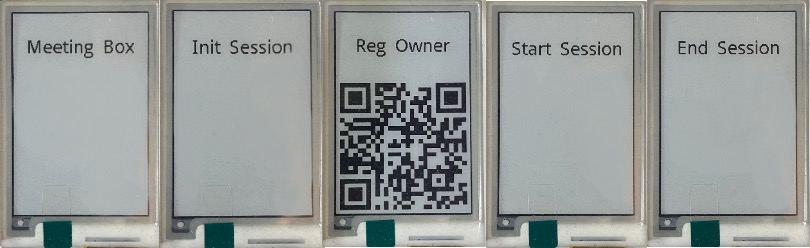
\includegraphics[width=1.0\textwidth]{epaper}
    \caption{電子紙於會談各階段之狀態顯示}\label{fig:epaper}
\end{figure}

\begin{figure}[H]
    \centering
    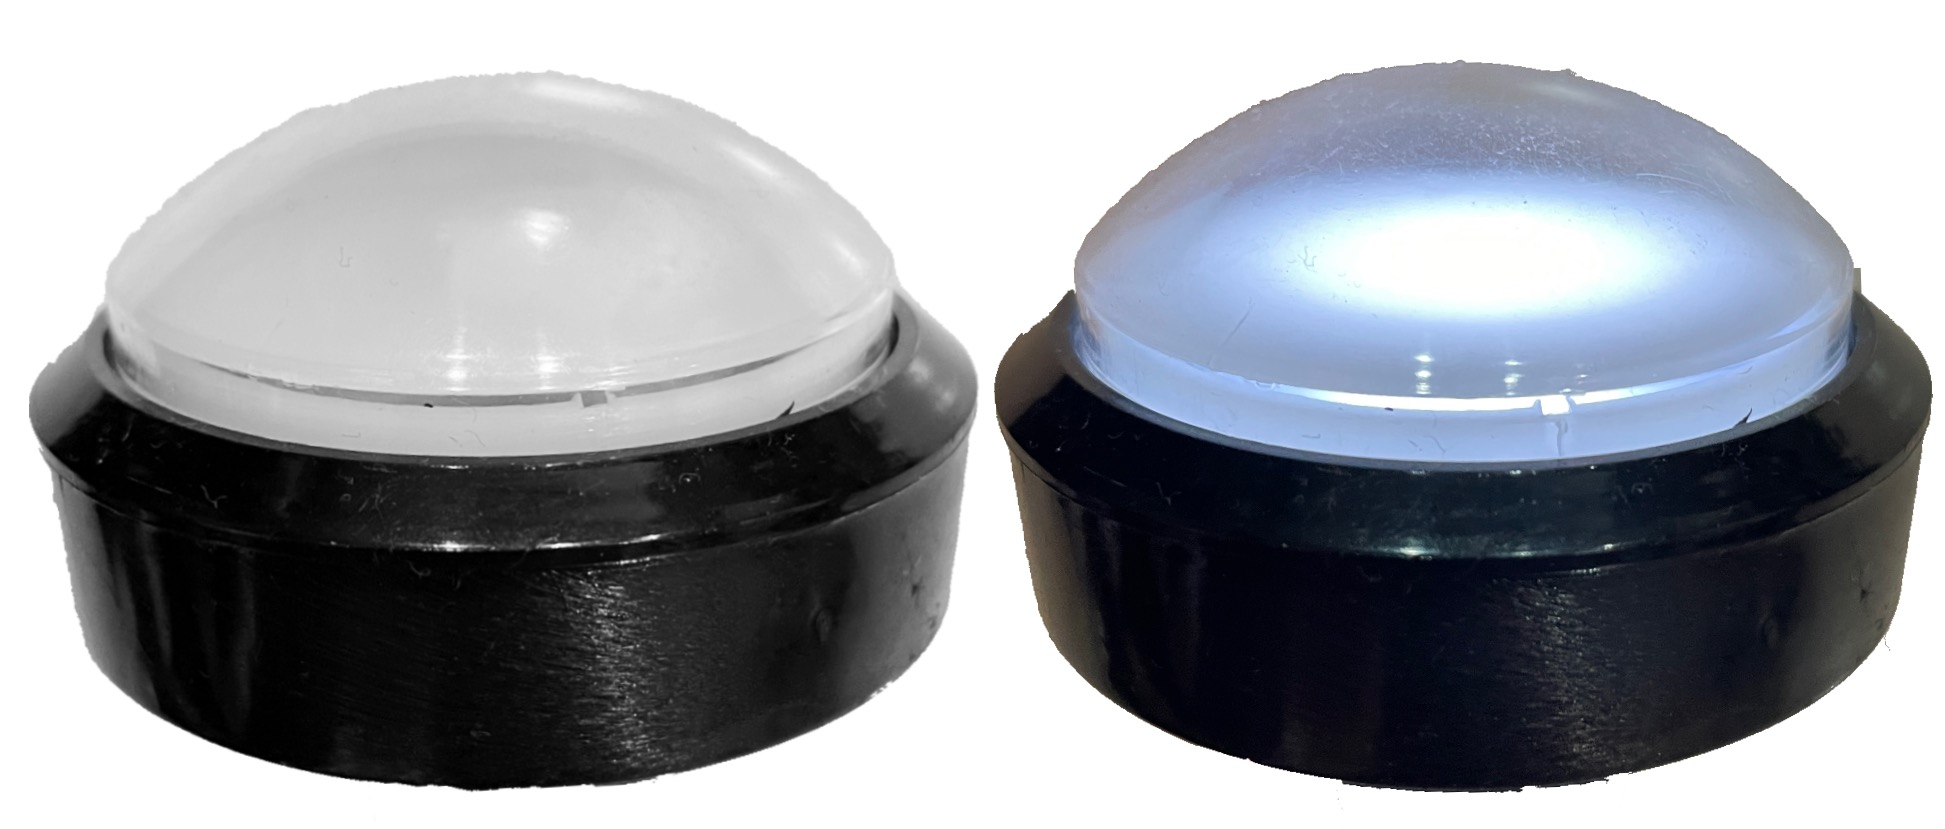
\includegraphics[width=0.5\textwidth]{btn}
    \caption{按鈕於會談開始/結束錄音之狀態指示燈}\label{fig:btn}
\end{figure}

\paragraph{運算控制核心與網路介面}

    如圖 \ref{fig:mbox} \nameref{fig:mbox}中右下綠色點線方框所示。
本系統實作以 Raspberry Pi 4B 為例,包含一 Geekworm X728 電池模組用於供電。
邏輯控制核心使用 Python 實作,控制周邊裝置包含人機互動介面、物理控制介面、超音波麥克風干擾器與錄音麥克風,
並網路介面與解封伺服器溝通。透過 GPIO 接收來自物理控制介面介面的外部觸發事件;透過 SPI 介面控制人機互動介面;
透過 GPIO 控制一外部 MOSFET 開啟關閉超音波干擾器;透過 fork/exec 呼叫 arecord 透過麥克風進行錄音;



\subsection{解封伺服器}

    本研究所設計之系統中解封伺服器的服務介面 RESTful\cite{fielding2000architectural} API 組成,
包含數個 API 端點,使用 Golang 搭配 Gin 網頁框架實作。
系統後端組件包含一資料庫 PostgreSQL 13 作為資料關聯綁定以及儲存的媒介;
包含 Docker 容器化執行引擎,用於封裝主動式噪音消除的 Python3 執行環境;
各 API 端點說明如下。

\begin{enumerate}
    \item \texttt{POST},~ \texttt{/meeting/}

        此 API 端點實作章節 \ref{sec:protocol} \nameref{sec:protocol}中,
    \nameref{subsec:protocol-init-create} 的 $M_{1}$ 、 $M_{2}$。
    當 API 端點收到請求後,會執行 \DEFfuncIDgen{} 與 \DEFfuncKgen{},
    分別產生此次會談的唯一識別碼 \DEFsessionID,與此次會談的解封金鑰 \DEFunsealKey。

        其中 \DEFfuncIDgen{} 為唯一識別碼產生函數,其產生須滿足唯一性、隨機性、不可預測性,
    本研究實作以 UUID \cite{rfc4122} 為例。
    \DEFfuncKgen{} 為對稱式加密演算法的金鑰產生函數,
    本研究實作以 AES CFB 模式 \cite{117146}\cite{9171} 為例。

    \item \texttt{POST},~ \texttt{/meeting/:id/owner}

        此 API 端點實作章節 \ref{sec:protocol} \nameref{sec:protocol}中,
    \nameref{subsec:protocol-init-reg} 的 $M_{3}^{i}$ 、 $M_{4}^{i}$。
    當 API 端點收到請求後,會執行 \DEFfuncPKgen{} 與 \DEFfuncIDgen{},
    分別產生一組屬於會談主持者 \DEFowner 的公開私密金鑰對 $($\DEFpublicKey$,~$ \DEFprivateKey$)$,
    與此會談主持者 \DEFowner 的唯一識別碼 \DEFownerID。

        其中會談主持者的唯一識別碼 \DEFownerID,其產生須滿足唯一性、隨機性、不可預測性,
    本研究實作以 UUID \cite{rfc4122} 為例。
    \DEFfuncPKgen{} 為非對稱加密演算法的公開私密金鑰對產生函數,
    本研究實作以 RSA PKCS\#1 \cite{rfc8017} 為例。
    路由變數 \texttt{:id} 為此次會談的唯一識別碼 \DEFsessionID。

    \item \texttt{POST},~ \texttt{/meeting/:id/end}

        此 API 端點實作章節 \ref{sec:protocol} \nameref{sec:protocol}中,
    \nameref{subsec:protocol-sessioning} 的 $M_{1}$ 、 $M_{2}$。
    當 API 端點收到請求後,主持者註冊人數 \DEFowreg 是否為一或多人,
    可能執行非對稱式金鑰演算法加密函數 \DEFfuncEncPK{} 或金鑰分割函數 \DEFfuncSSS{}。

        其中 \DEFfuncEncPK{} 為非對稱式金鑰演算法加密函數,本研究實作以 RSA PKCS\#1 \cite{rfc8017} 為例。
    \DEFfuncSSS{} 為金鑰分割函數,
    本研究實作以 Shamir's Secret Sharing \cite{shamir1979share} 於 $GF(2^8)$ 的實作 \cite{117146} 為例。
    路由變數 \texttt{:id} 為此次會談的唯一識別碼 \DEFsessionID。

    \item \texttt{POST},~ \texttt{/unseal/:id/rec/:kind}

        此 API 端點實作根據路由中變數 \texttt{:kind} 可能為章節 \ref{sec:protocol} \nameref{sec:protocol}中,
    \nameref{subsec:protocol-init-create} 的 $M_{3}$ 、 $M_{4}$,
    或章節 \ref{sec:protocol} \nameref{sec:protocol}中,
    \nameref{subsec:protocol-sessioning} 的 $M_{3}$ 、 $M_{4}$。
    其功能皆為上傳錄音,透過判斷路由中變數 \texttt{:kind} 得知上傳的是何種錄音,
    執行關聯綁定屬於此次會談的唯一識別碼 \DEFsessionID。
    路由變數 \texttt{:id} 為此次會談的唯一識別碼 \DEFsessionID。

    \item \texttt{GET},~ \texttt{/unseal/:meetingid/:ownerid}

        此 API 端點實作章節 \ref{sec:protocol} \nameref{sec:protocol}中,
    \nameref{subsec:protocol-unseal-auth} 的 $M_{1}^{i}$ 、 $M_{2}^{i}$。
    路由變數 \texttt{:meetingid} 為此次會談的唯一識別碼 \DEFsessionID。
    路由變數 \texttt{:ownerid} 為會談主持者唯一識別碼 \DEFownerID。

    \item \texttt{PUT},~ \texttt{/unseal/:meetingid/:ownerid}

        此 API 端點實作章節 \ref{sec:protocol} \nameref{sec:protocol}中,
    \nameref{subsec:protocol-unseal-auth} 的 $M_{3}^{i}$ 、 $M_{4}^{i}$。
    會談主持者的私密金鑰 \DEFprivateKey,透過非對稱式加密演算法之解密函數 \DEFfuncDecSK{},
    將受加密保護的授權金鑰 \DEFakEnc 解密,接著使用同一會談主持者的私密金鑰 \DEFprivateKey,
    透過數位簽章演算法簽之簽名函數 \DEFfuncSignSK{}。
    解封伺服器 \DEFserver 使用會談主持者的公開金鑰 \DEFpublicKey,
    透過數位簽章演算法簽之驗證函數 \DEFfuncVerfPK{},驗證解密後的授權金鑰與其簽名。

        其中 \DEFfuncDecSK{} 為非對稱式加密演算法之解密函數;\DEFfuncSignSK{} 為數位簽章演算法簽之簽名函數;
    \DEFfuncVerfPK{} 為過數位簽章演算法簽之驗證函數;本研究實作以 RSA PKCS\#1 \cite{rfc8017} 為例。
    路由變數 \texttt{:meetingid} 為此次會談的唯一識別碼 \DEFsessionID。
    路由變數 \texttt{:ownerid} 為會談主持者唯一識別碼 \DEFownerID。

    \item \texttt{GET},~ \texttt{/unseal/:meetingid/access}

        此 API 端點實作章節 \ref{sec:protocol} \nameref{sec:protocol}中,
    \nameref{subsec:protocol-unseal-access} 的 $M_{1}$ 、 $M_{2}$。
    當 API 端點收到請求後,主持者註冊人數 \DEFowreg 是否為一或多人,
    可能執行對稱式加密演算法之解密函數 \DEFfuncDecEK{} 或金鑰分割演算法合併函數 \DEFfuncSSC{}。
    接著透過聲音樣本的離散時間誤差推估函數 \DEFfuncEstm{},得到兩聲音樣本的離散時間對齊誤差值 \DEFshift。
    再透過自適應噪音消除 \DEFfuncAnc{},還原獲得有效的會談聲音記錄 \DEFrecREV。

        其中 \DEFfuncDecEK{} 對稱式加密演算法之解密函數,
    為本研究實作以 AES CFB 模式 \cite{117146}\cite{9171} 為例。
    \DEFfuncSSC{} 為金鑰分割演算法合併函數。
    本研究實作以 Shamir's Secret Sharing \cite{shamir1979share} 於 $GF(2^8)$ 的實作 \cite{117146} 為例。
    路由變數 \texttt{:meetingid} 為此次會談的唯一識別碼 \DEFsessionID。

        其中 \DEFfuncEstm{} 離散時間誤差推估函數,透過 \texttt{goroutine} 於背景中執行。
    此為 Golang 的輕量執行緒,此函式呼叫為非阻塞式呼叫。
    \DEFfuncAnc{} 為自適應噪音消除函數,
    本研究實作以引用 M Cejnek 的自適應訊號處理開源函式庫 \cite{cejnek2017padasip} 為例。
    透過 Docker 於容器環境 \texttt{jupyter/scipy-notebook} 中執行。
    此呼叫利用 \texttt{goroutine} 於背景中執行,為非阻塞式呼叫。
\end{enumerate}


\subsection{行動應用程式}

    會談主持者持有智慧型裝置,且透過行動應用程式(mobile application)與會談終端互動,獲取會談終端上的資訊。
並有能力於各階端包含會談初始化、會談進行中、談結束後,與解封伺服器進行通訊。
本研究實作以單頁應用(Single-page Application, SPA)為例。

\begin{figure}[H]
    \centering
    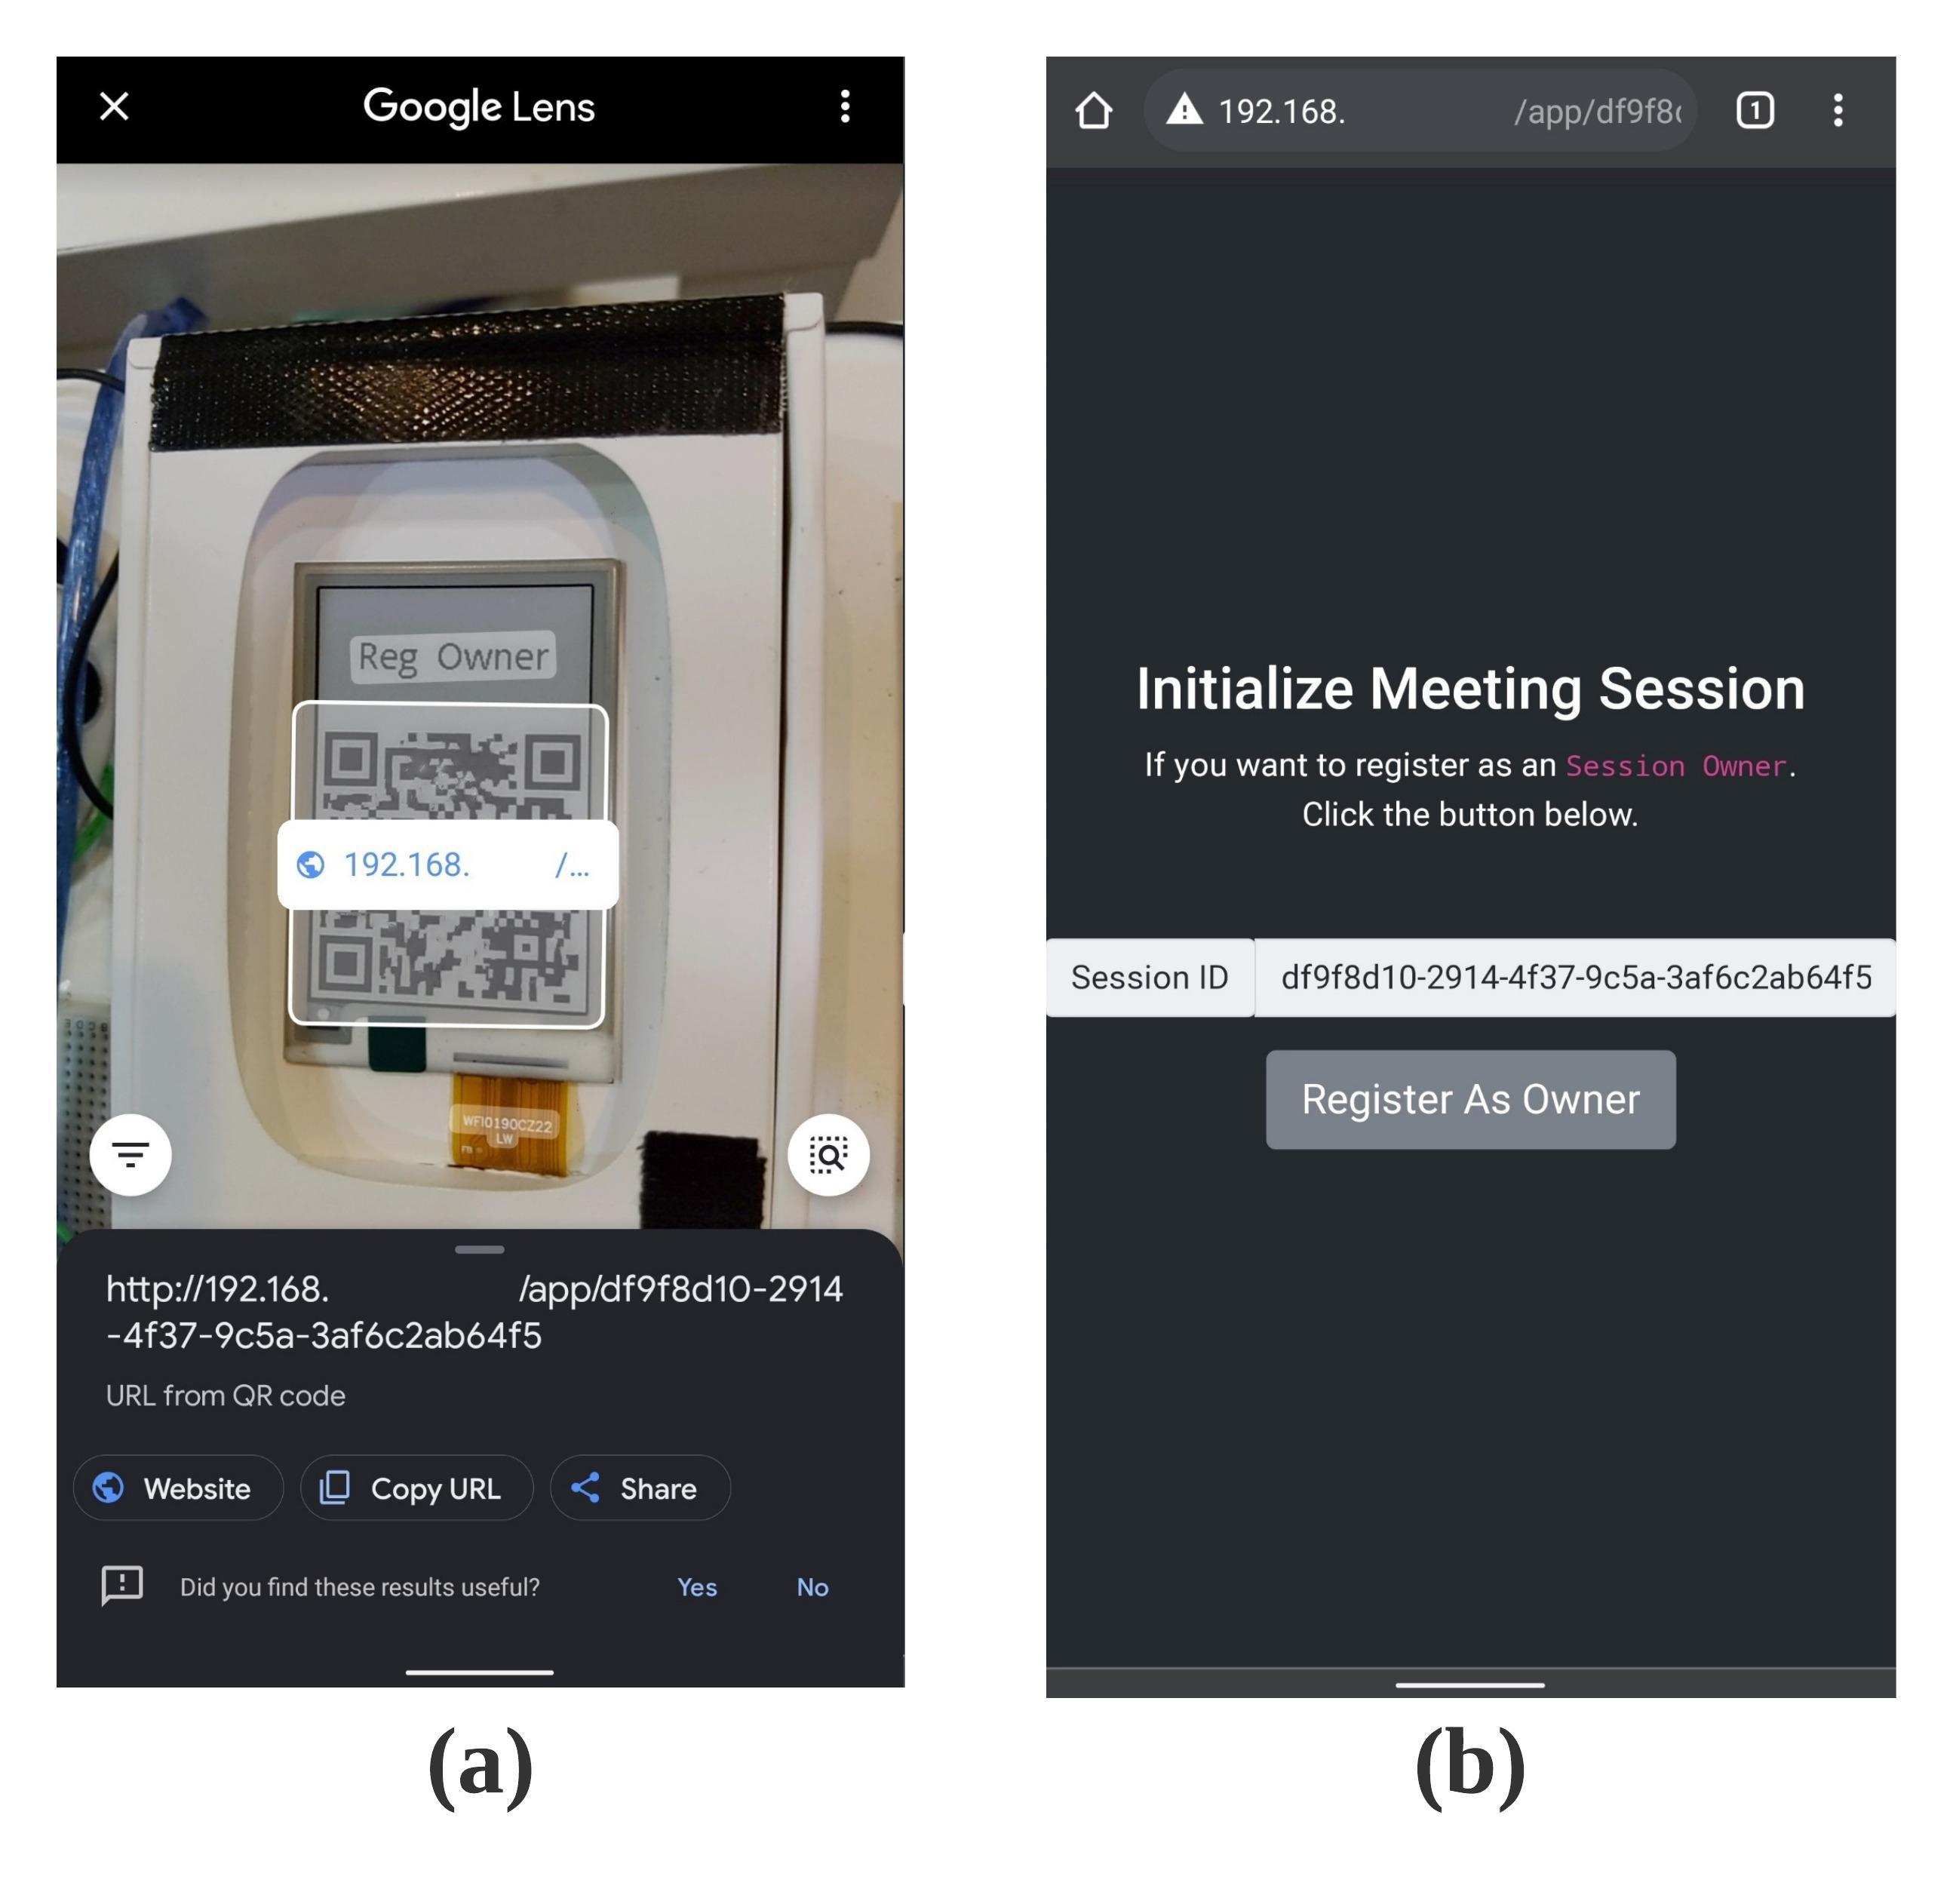
\includegraphics[width=0.6\textwidth]{app-1}
    \caption{行動應用程式會談初始化使用者介面}\label{fig:app-1}
\end{figure}

\begin{figure}[H]
    \centering
    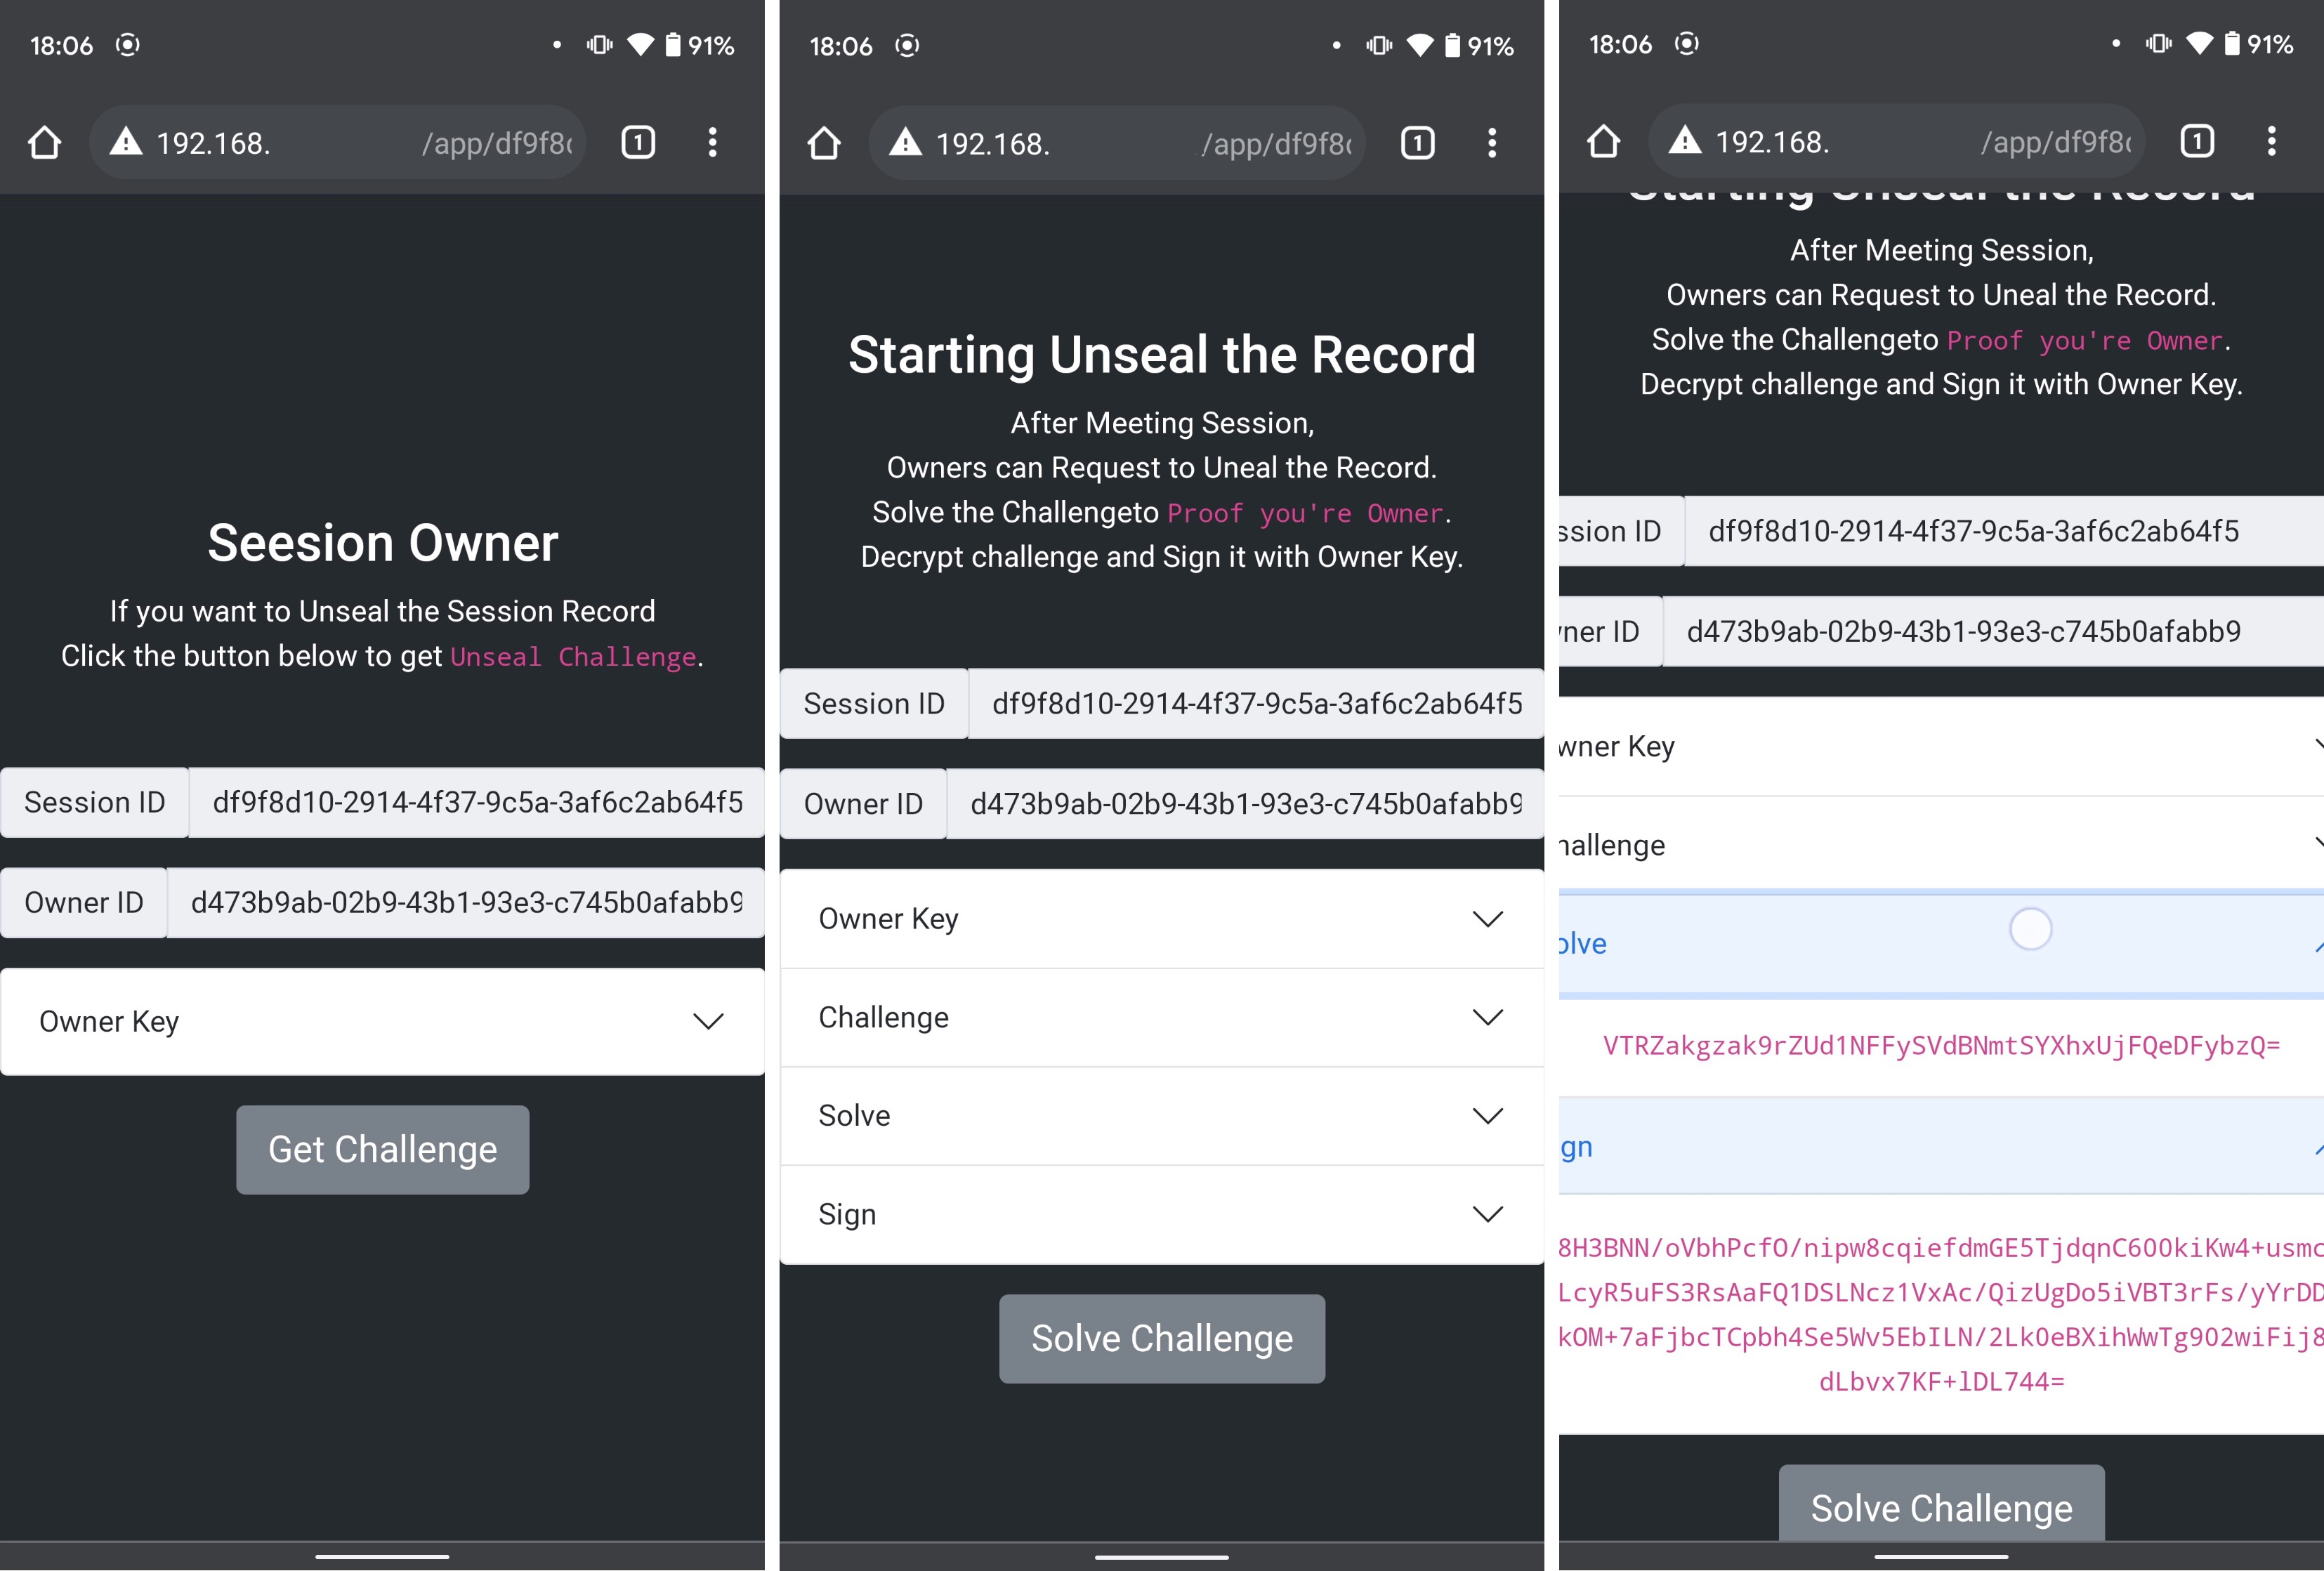
\includegraphics[width=0.85\textwidth]{app-2}
    \caption{行動應用程式會談主持者授權解封伺服器使用者介面}\label{fig:app-2}
\end{figure}

\begin{figure}[H]
    \centering
    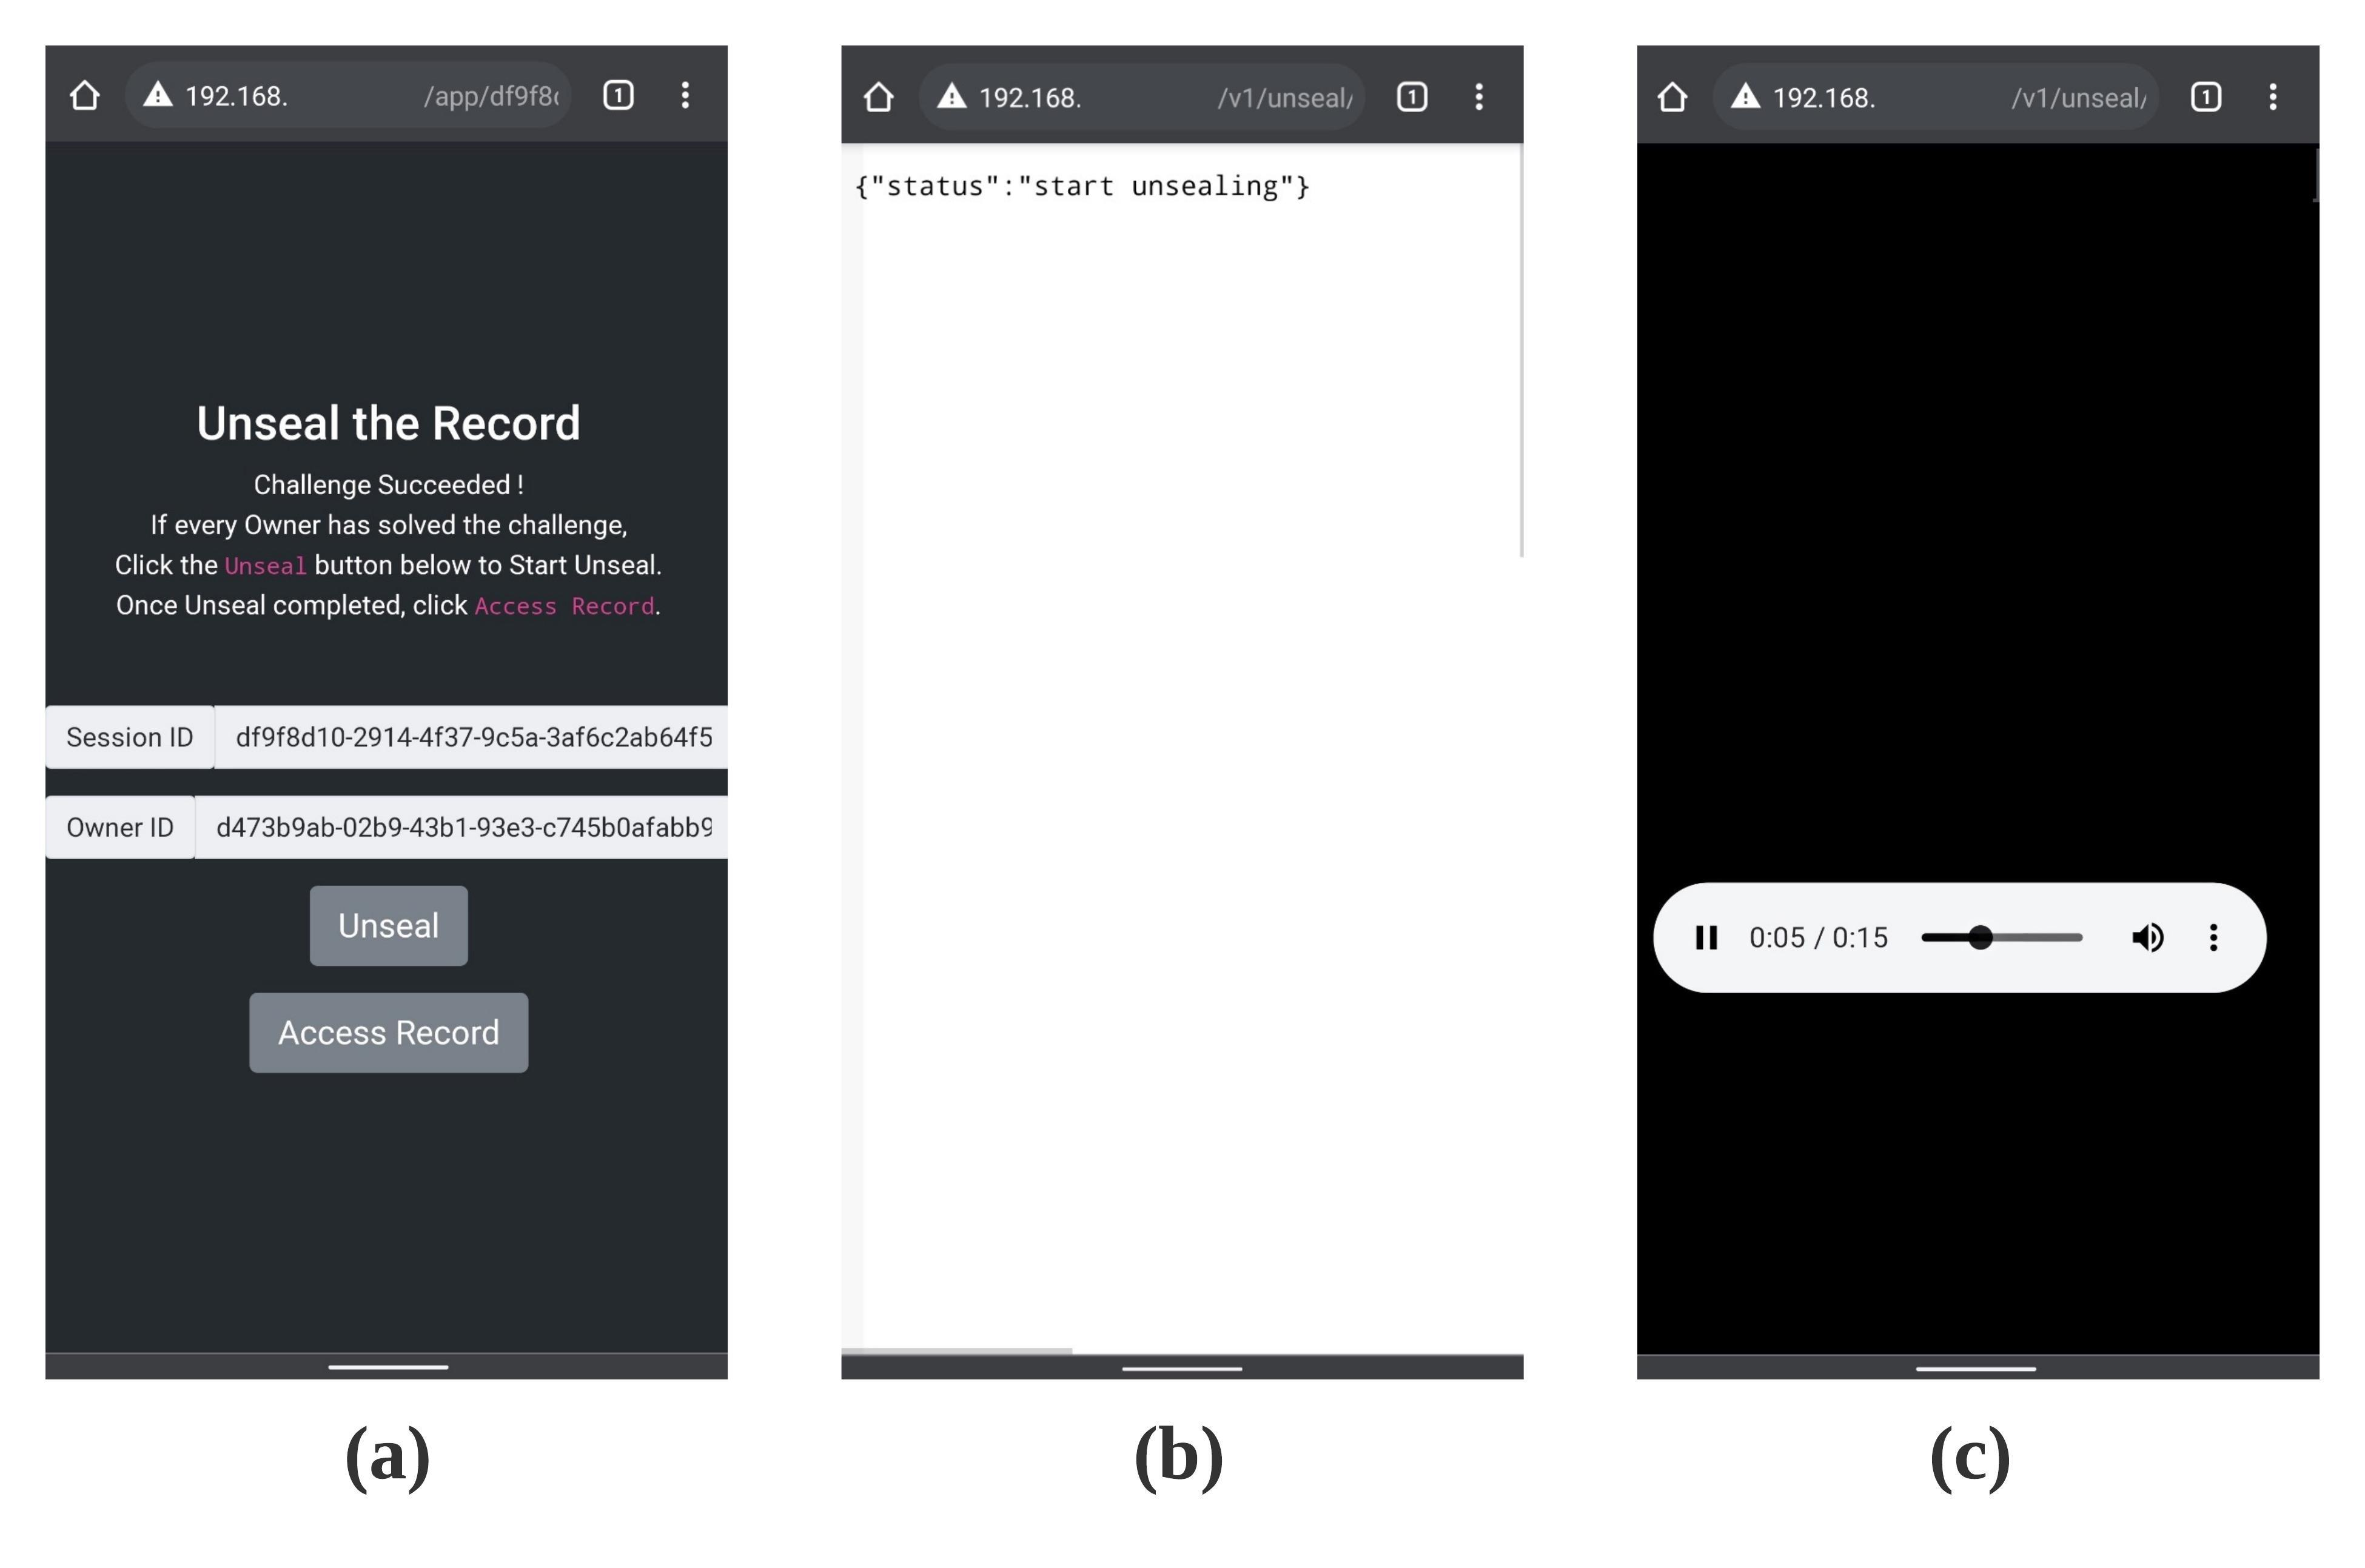
\includegraphics[width=0.85\textwidth]{app-3}
    \caption{行動應用程式取得會談聲音記錄使用者介面}\label{fig:app-3}
\end{figure}


\section{系統實驗}

\subsection{超音波麥克風干擾器之干擾效果分析}

    會談聲音與麥克風干擾器產生的干擾之信噪比下,干擾效果的分析。
包含人耳聽感,與語音識別。


\subsection{主動式噪音消除效果分析}

    會談聲音與麥克風干擾器產生的干擾之信噪比下,噪音消除效果分析。
包含人耳聽感,與語音識別。


\subsection{聲音樣本離散時間推估演算法}

    此演算法的執行前後聲波比對圖,與執行過程數值的變化。


\subsection{解封會談聲音記錄分析性能分析}

    伺服器獲得授權後,執行聲音樣本離散時間推估演算法與主動式噪音消除來還原產生有效的會談聲音紀錄,
其錄音長度與執行時間的時間複雜度性能分析。


\section{實驗結果與討論}

    本研究所設計之系統可以確保 Server 在 Running {\it Meeting Session}結束後,
直到成功解封 ({\it Unseal})之前,\DEFrecREV 保有機密性。

\begin{figure}[H]
    \centering
    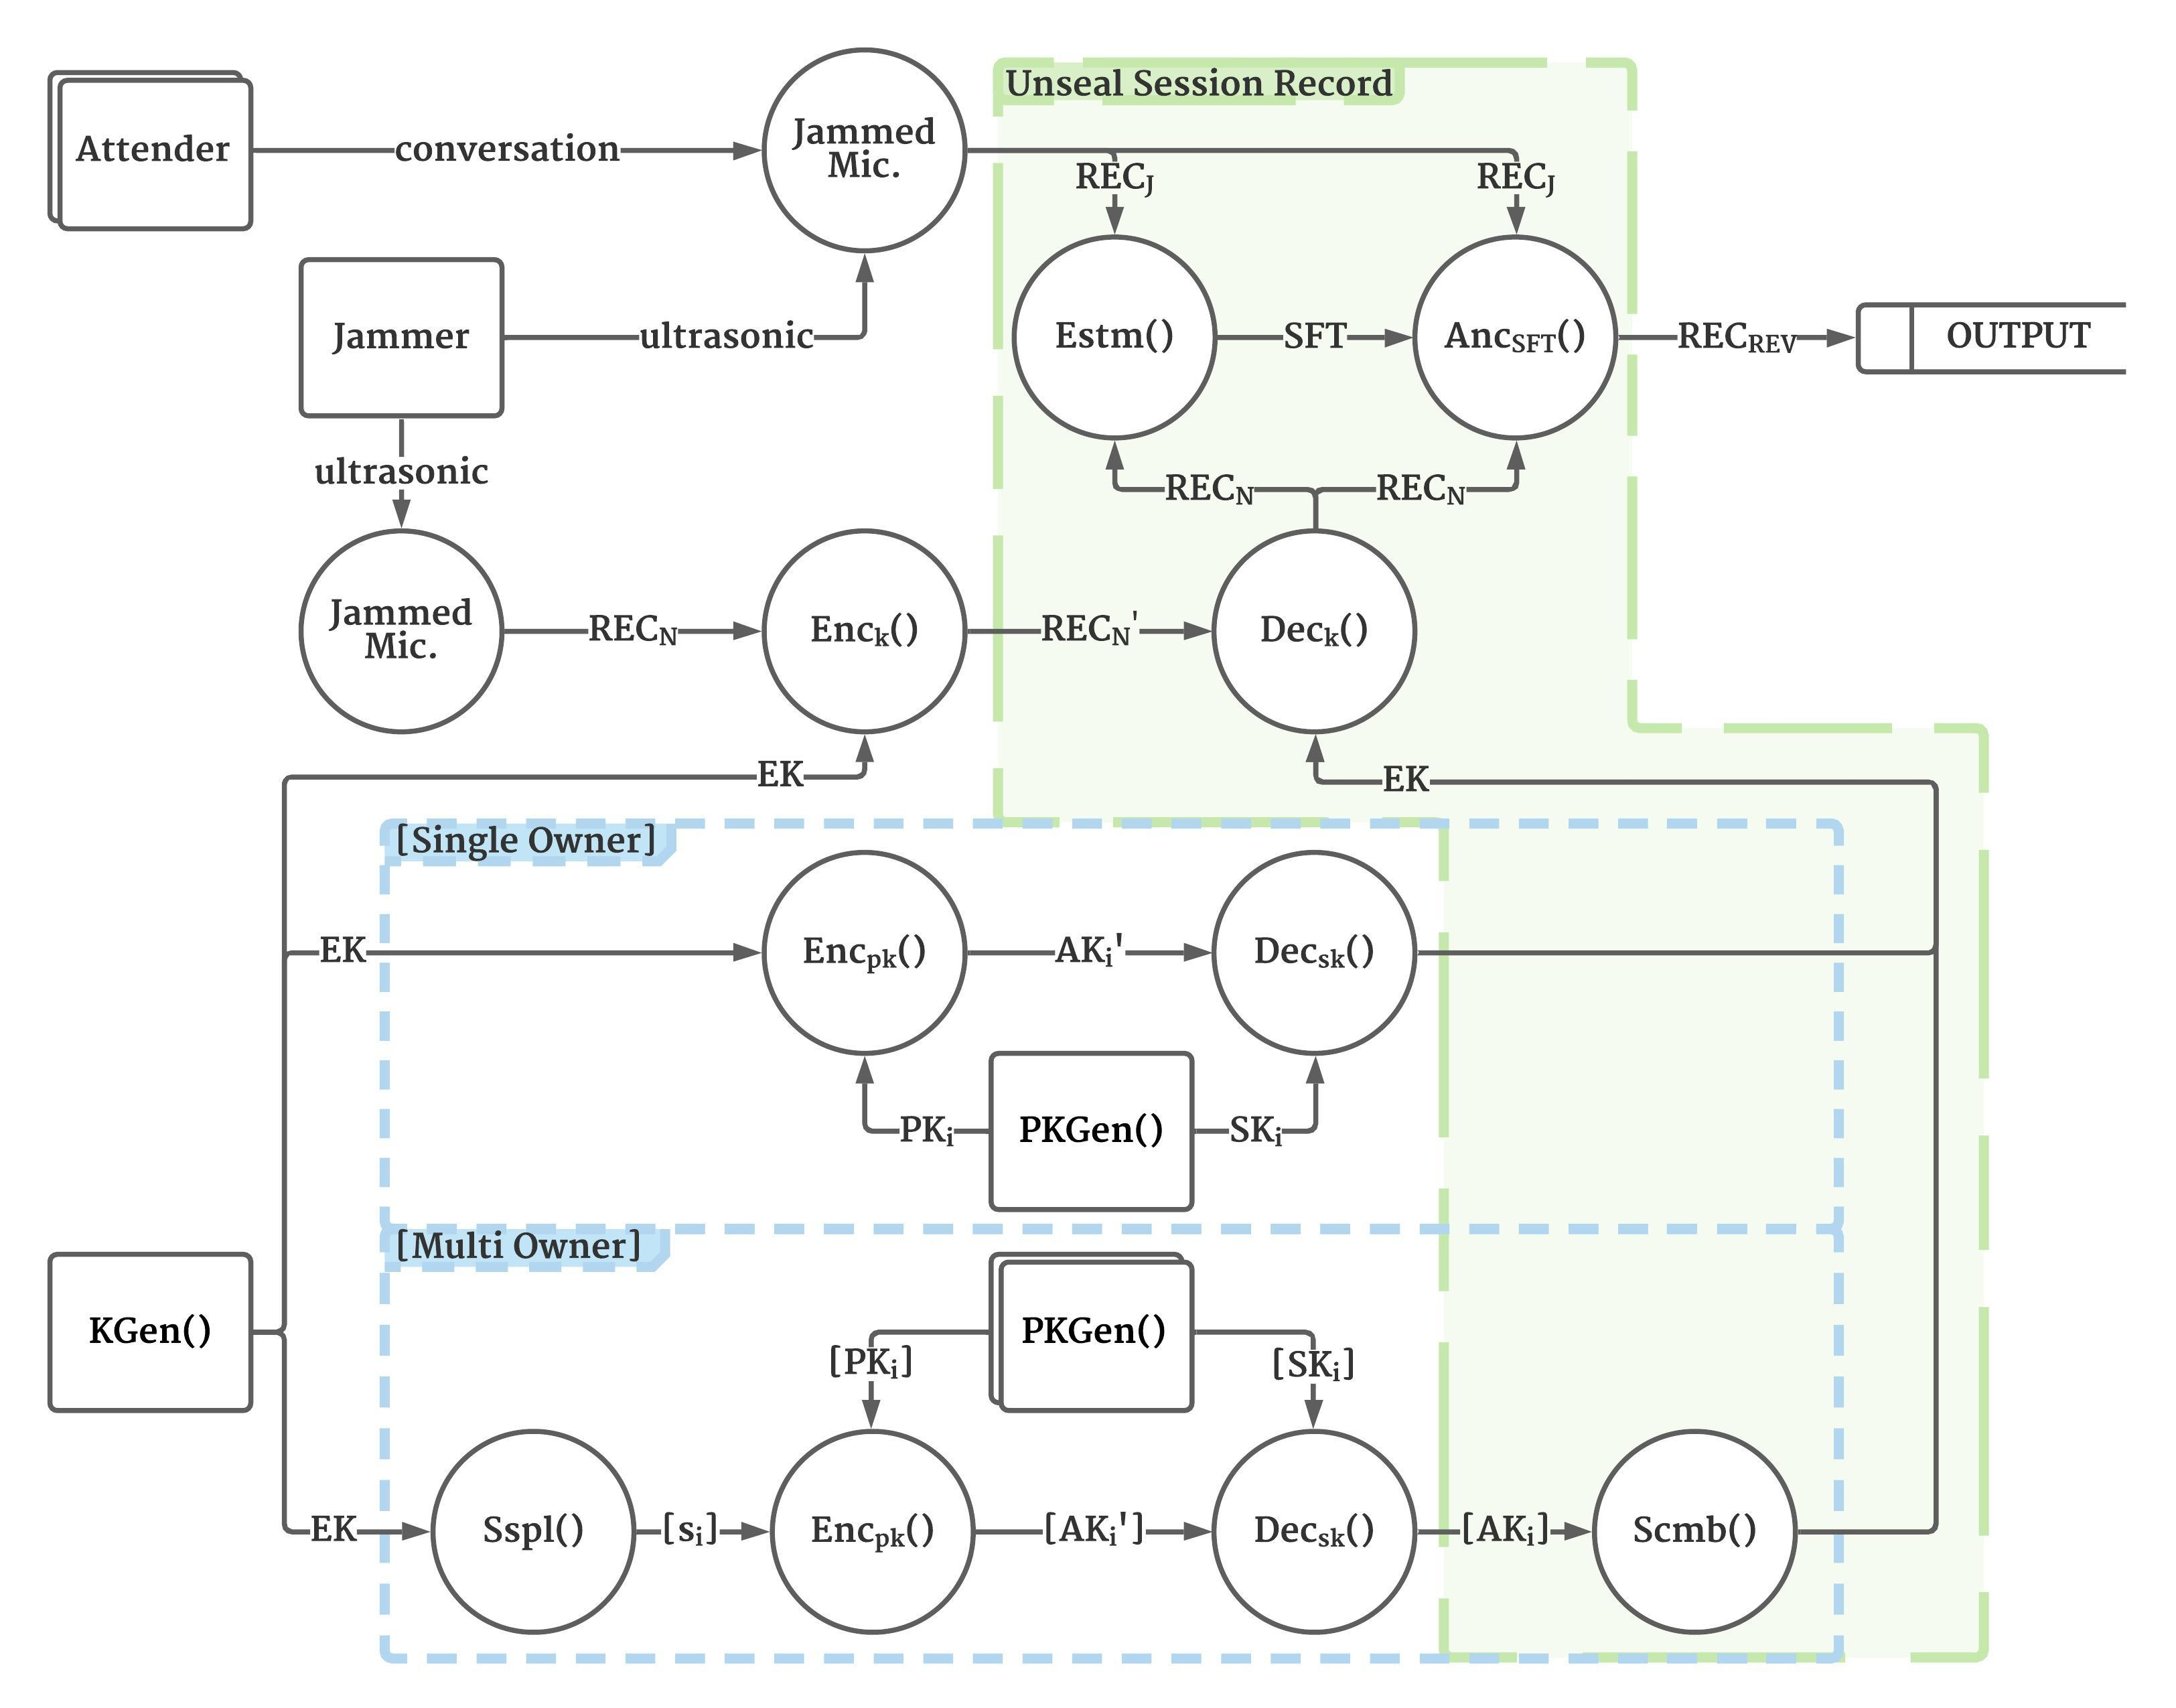
\includegraphics[width=1.0\textwidth]{system-data-flow}
    \caption{系統資料流程圖}\label{fig:system-data-flow}
\end{figure}